\section{Travaux de modélisations} 
\subsection{Modification du Modèle Conceptuelle de Donnée}

Pour permettre l'enregistrement des lieux d'emprunts des différents emprunts il a fallu ajouter une table lieu d'emprunt au MCD déjà existant dans Royal\_.
\begin{wrapfigure}[1]{l}{12cm}
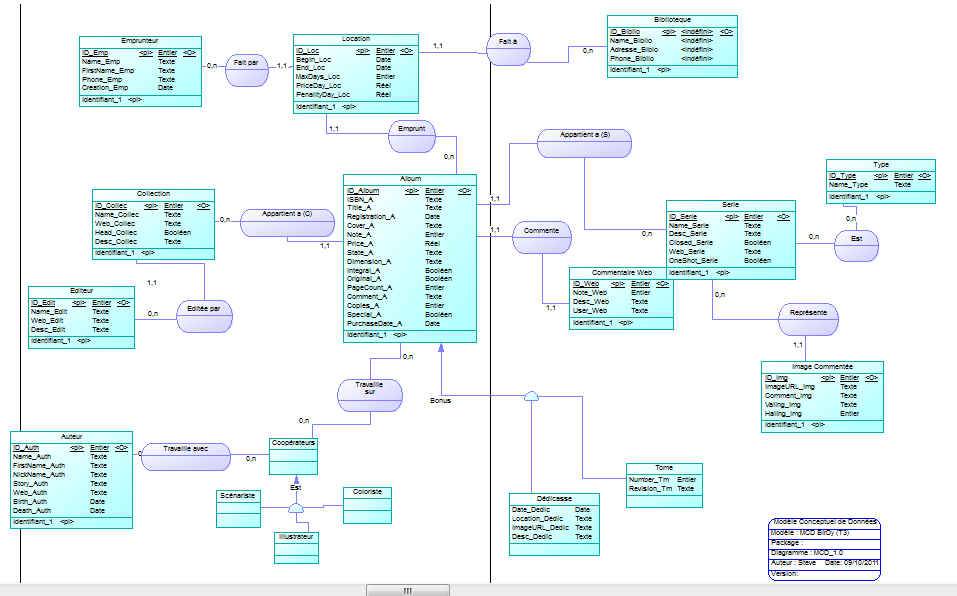
\includegraphics[width=12cm]{MCD_Royal_Modif.png}
\end{wrapfigure}
\clearpage{}

\subsection{Diagrammes d'activités}

\section{Travaux de modélisations}

\subsection{Diagrammes d'activités}

\begin{figure}[h!]
\begin{center}
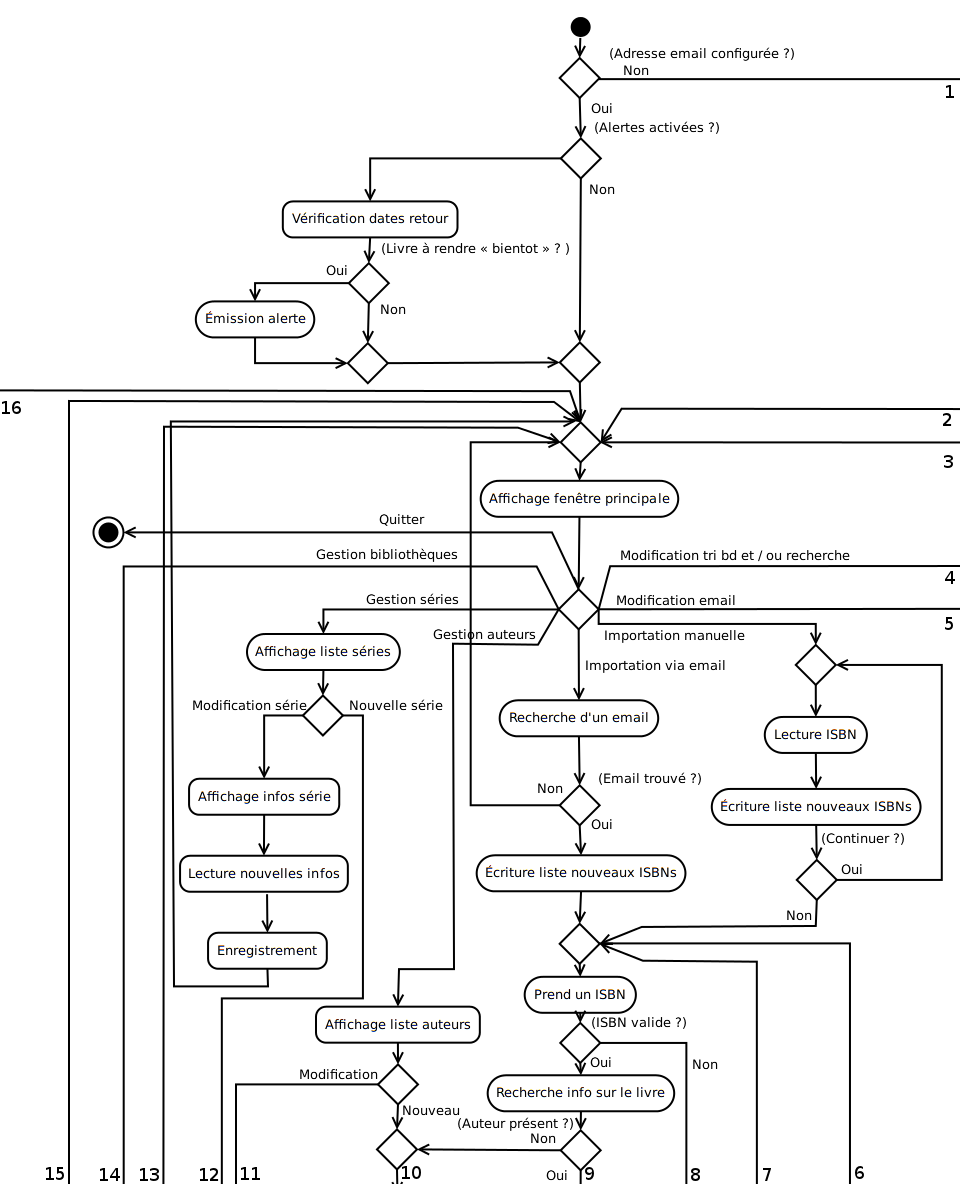
\includegraphics[width=16cm, height=19cm]{uml/appli_pc/p1.png}
\end{center}
\end{figure}
\newpage{}

\begin{figure}[h!]
\begin{center}
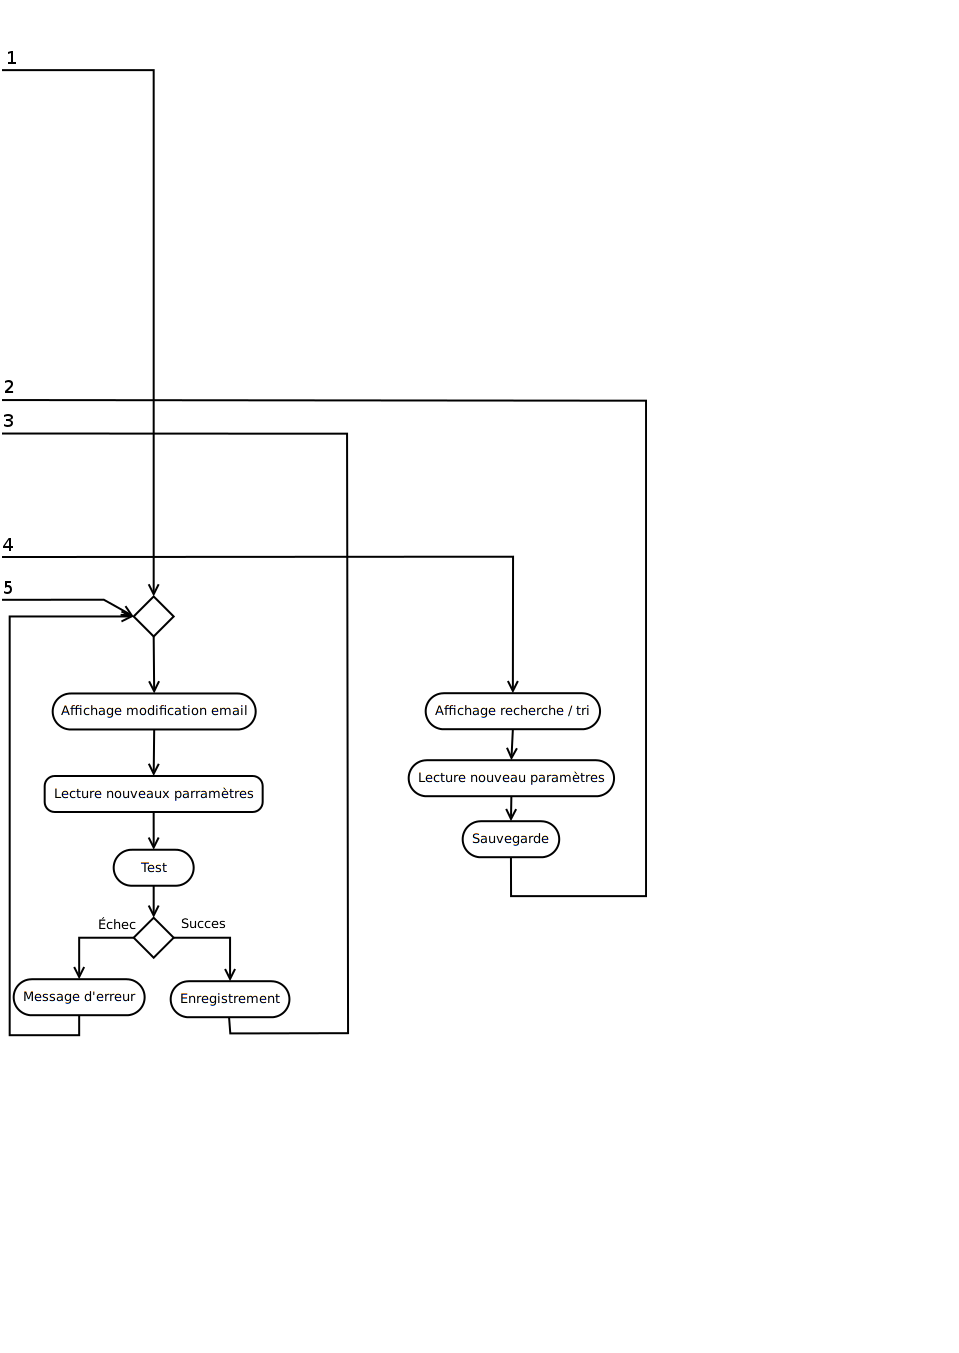
\includegraphics[width=16cm]{uml/appli_pc/p2.png}
\end{center}
\end{figure}
\newpage{}

\begin{figure}[h!]
\begin{center}
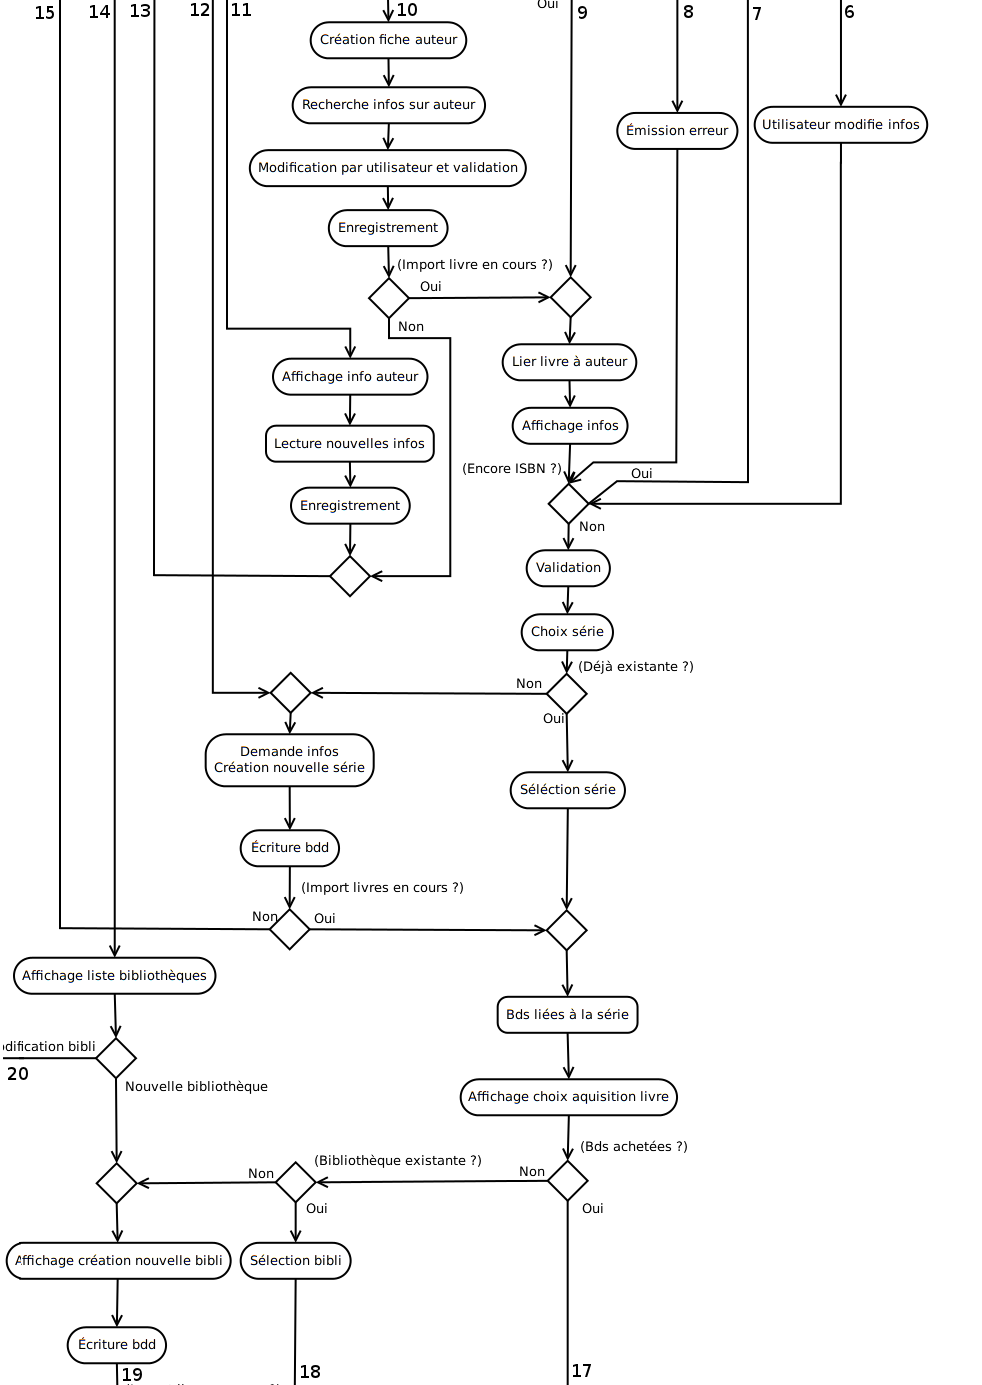
\includegraphics[width=16cm]{uml/appli_pc/p3.png}
\end{center}
\end{figure}
\newpage{}

\begin{figure}[t!]
\begin{center}

\includegraphics[width=16cm]{uml/appli_pc/p4.png}
\end{center}
\end{figure}

Une version plus lisible est disponnible à l'adresse suivante : 
\emph{www.spyzone.fr/modules/images/pc_application.png}

